In this subsection, we will present varied ways to visualize the network and some techniques to improve the visualization by using the attributes of the edges and nodes.

\begin{figure}[ht]
\centering
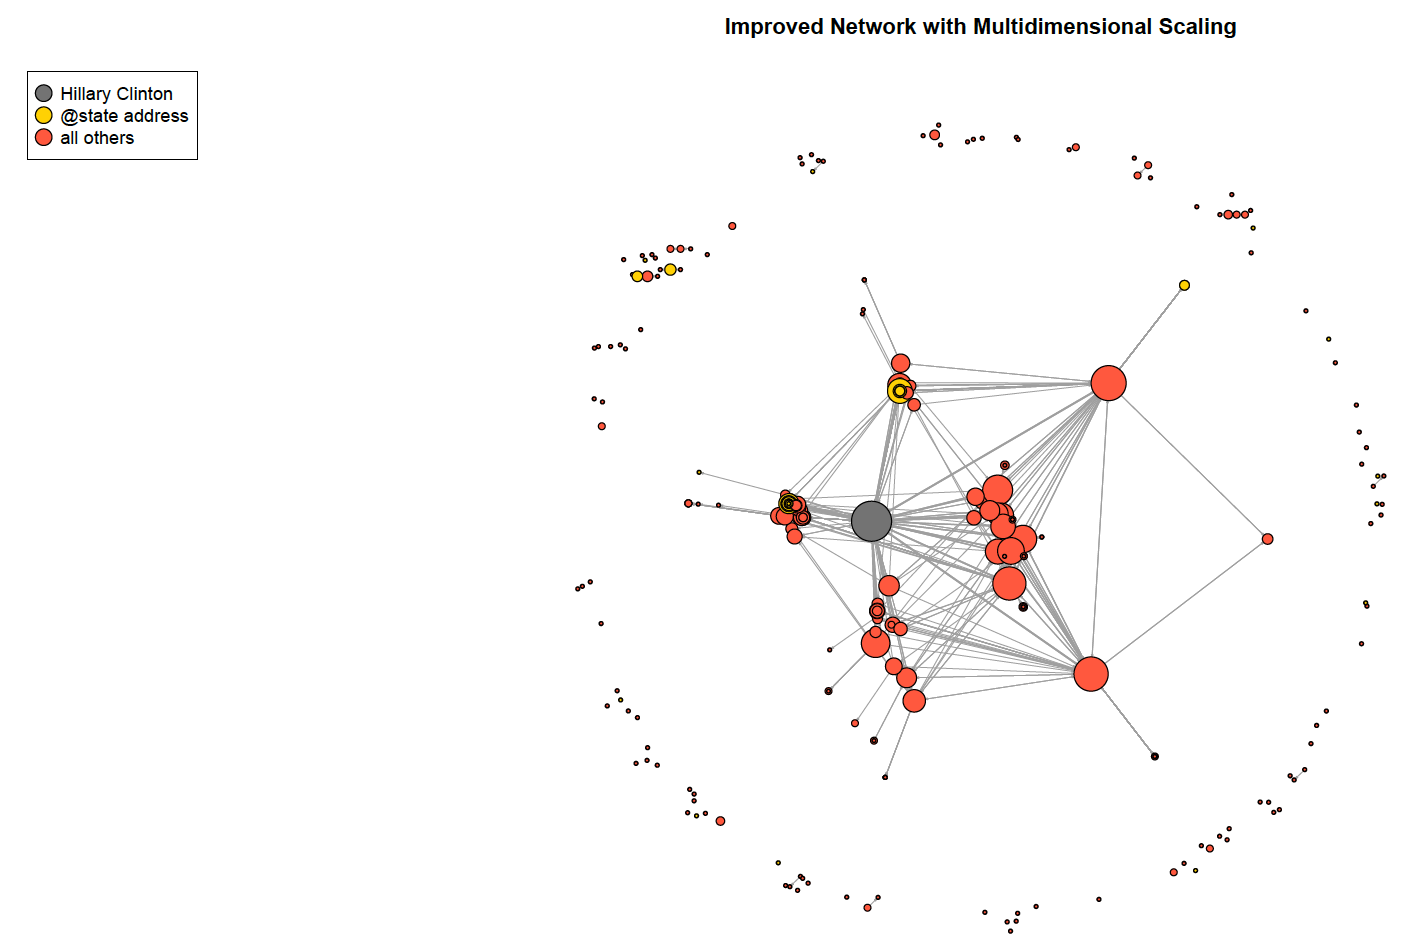
\includegraphics[width = 1\textwidth]{zoe/report_dms_layout}
\label{fig:improvednw}
\caption{Improved Network after Deleting Low-weight Edges}
\end{figure}

One key factor for effective visualization of a network is the graph layout. We have compared $15$ different types of layout and decided to display our network with the Multidimensional Scale layout. The algorithm behind each layout scheme is beyond the scope of our discussion in this report, but we do invite the readers to see Appendix \ref{App:AppendixB}  and compare all $15$ layouts we have tested.

The natural choice of color and size for nodes is based on the values of variables ``\verb+person_type+'' and ``\verb+active_size+''. See the legend in Figure \ref{fig:improvednw} to understand the colorcode. Table \ref{tab:node_size} in the previous subsection suggests the distribution of node size is highly skewed, hence we need to rescale it to make it i) more reasonable as iGraph object input as the default is $15$ and ii) have less variance. Inspired by the variance-stablizing transformation, we devised the following rescaling scheme in Equation (\ref{eqt:rescale}). The side-by-side histograms in Figure \ref{fig:rescalenode} demonstrates that this rescaling scheme is effective. The similary log-transform rescaling was also applied to the edge weight, which is also highly skewed.
\begin{equation}
\label{eqt:rescale}
\verb+rescaled active_size+ = \log \verb+active_size+ + 1
\end{equation}

\begin{figure}[ht]
\centering
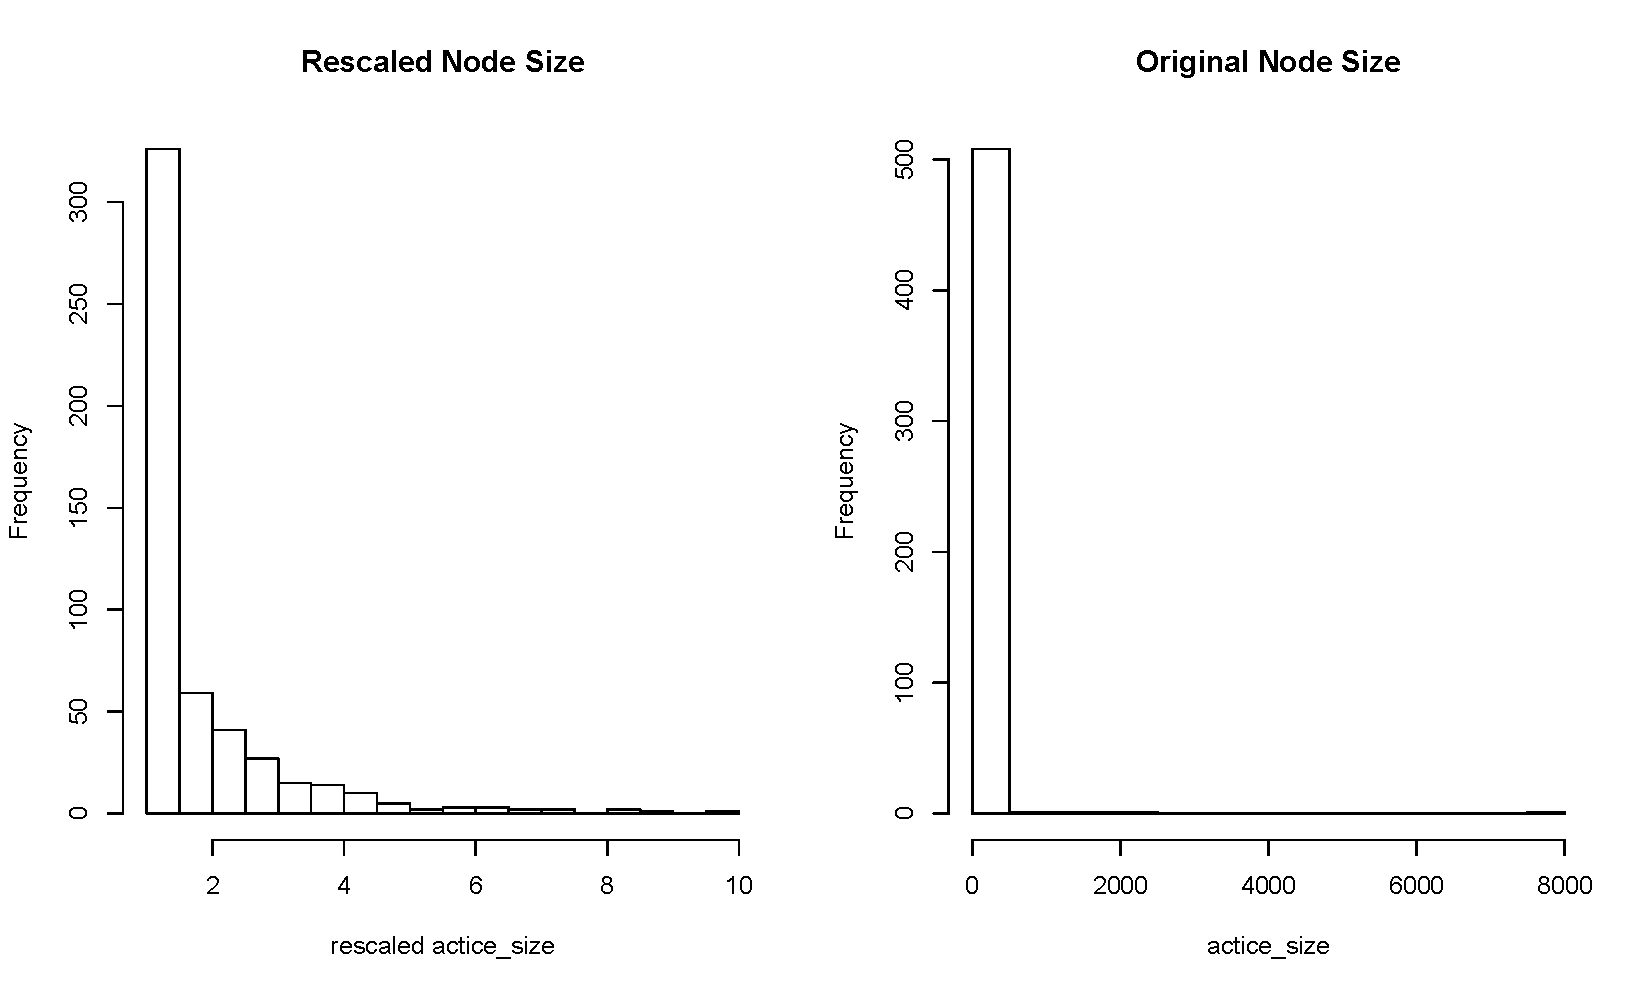
\includegraphics[width=.9\textwidth]{zoe/report_rescaled_size}
\caption{Rescaling of Node Size}
\label{fig:rescalenode}
\end{figure}

\begin{figure}[ht]
\centering
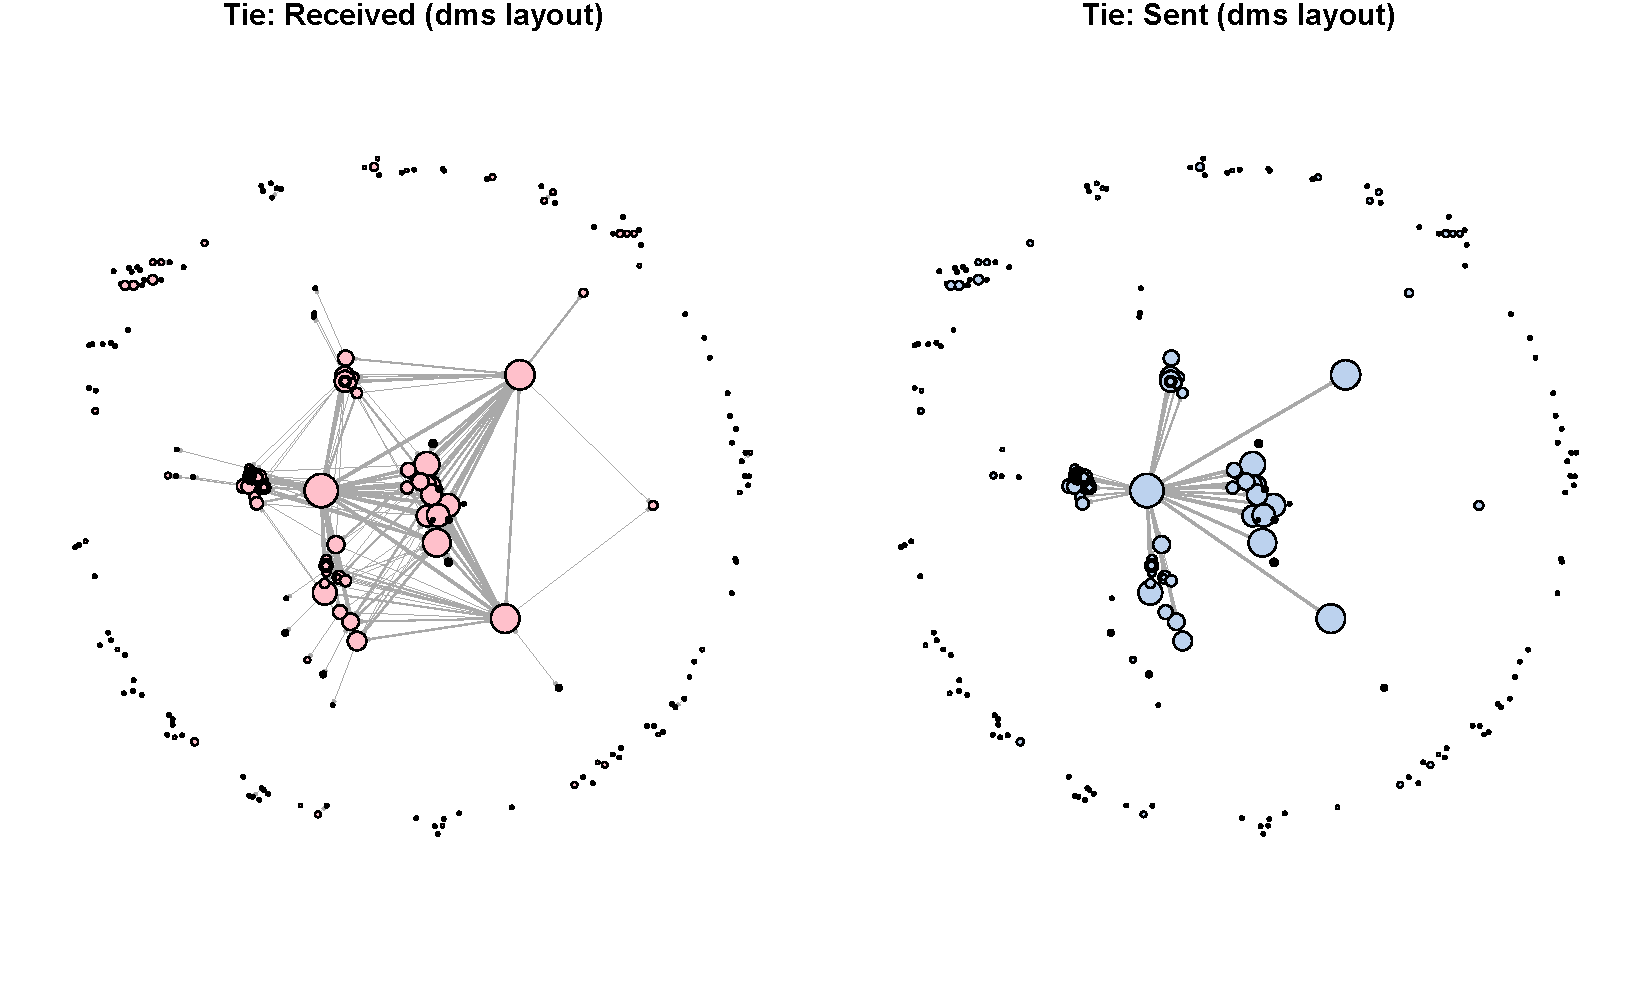
\includegraphics[width=.9\textwidth]{zoe/report_network_compare}
\caption{Visualizing Hillary Clinton Received and Sent E-mails}
\label{fig:splitnw}
\end{figure}

Given a Hillary-centric network, we are also interested in examining the network by looking at the e-mails she received and sent separately. Figure \ref{fig:splitnw} shows the side-by-side sub-networks, split by receiving and sending.
